%************************************************
\chapter{Introduction}\label{ch:introduction}
%************************************************
Coordination in \acf{DR} operations such as \acf{USAR} can be very challenging. In large-scale disasters, \ac{DR} teams may have limited resource and personnels to deal with multiple incidents across a large impact area. Task planning and execution need to be carried out by geographically distributed \ac{DR} teams in real time against uncertainties in the environment. The challenges highlight the opportunity space of technology support for real time task planning and execution.  \\ 

Recently, various \acf{ICT}, ranging from communication infrastructures to social media platforms, have been playing increasingly significant roles in  disaster management.  Moreover, \acf{MAS} researchers have devised various real-time task planning algorithms to automate planning in time critical task domains such as disaster response. The advances in both \ac{ICT} and Multi-agent optimisation algorithms lead to the opportunity of automated planning support in the \ac{DR} domain. However, before we apply these algorithm to support \ac{DR} operations, we need to understand how can we design the interaction between responder teams and the planning support in a way that improves, rather than hinders team performance. Empirical studies of \acf{CSCW} systems have shown that it is vital to study technology in use to understand potential tensions between social and technical aspects of a system. In particular, field studies of workflow support systems have revealed that technologies can disrupt rather than smooth workflow if they are not designed in a socially acceptable way. The aim of this work is to explore potential socio-technical issues surrounding a planning support system, which in turn, informs interaction design of such systems. \\

This PhD work is sponsored by the ORCHID research project(EPSRC grant), which contributes to the understanding needed to build \acf{HACS} in the disaster domain. As computational systems  becoming increasingly embedded into our life, the researchers from the ORDHID project envision a future in which people and computational agents operate at a global scale, forming human agent collectives. The ORCHID project aims to realise the vision of \ac{HACS} by studying the science that is needed to understand, build and apply \ac{HACS} that symbiotically interleave human and computer systems \footnote{www.orchid.ac.uk}.\\

This chapter will give an overview of the PhD work, which covers research objectives, approach, research questions and contributions, followed by a list of publications related to this thesis and an overview of the thesis structure.\\


\section{Problem Definition and Objectives}
In large scale disasters, a \ac{DR} team may have limited resources and personnel to deal with large number of incidents across a large geographic area under time pressure. In this situation, task and team allocation become a grand challenge for the \ac{DR} team. The responders and resources need to be assigned to teams and tasks in a way that minimises loss of life and costs (e.g., time or money). For instance responders with different capabilities (e.g., fire-fighting or life support) have to form teams in order to perform rescue tasks (e.g., extinguishing a fire or providing first aid). Thus, responders have to plan their paths to the tasks (as these may be distributed in space) and form specific teams to complete them. These teams, in turn, may need to disband and reform in different configurations to complete new tasks, taking into account the status of the current tasks (e.g., health of victims or building fire) and the environment (e.g., if a fire or radioactive cloud is spreading). Furthermore, uncertainty in the environment (e.g., road connectivity, task status update) or in the responders abilities to complete tasks (e.g., some may be tired or get hurt) means that plans are likely to change continually to reflect the prevailing assessment of the situation.\\

Recent advances in multi-agent systems research leads to a number of real-time simulation and optimization technologies, some of which have great potential to be adapted to support task planning for \ac{DR} teams (Section \ref{sec:lraisupport}). Although the opportunity space has been recognised, most multi-agent coordination algorithms have only been tested in computational simulations. None of them have been deployed to guide real human in \ac{DR} situations. However, extreme difficulties might be encountered when introducing new technology support for human teams. New technologies might not support, but might disrupt smooth workflow if they are designed in an organisationally unacceptable way. Much literature in \ac{CSCW} has pointed out how ill-designed work-flow management/automation system can lead to undesirable results, not only failing to improve work efficiency but also hindering human performance. Field studies of \ac{CSCW} technologies have shown that it is vital to study technology in use to understand potential tensions raised for teamwork. \\

This PhD work adopts a socio-technical view on the responder teams and their technological supporting systems. The term socio-technical system is used to describe a system that involves a complex interaction between humans, machines and the environmental aspects of the work system (Section \ref{sec:LRSocialTechnical}). Particularly, the interactional issues of planning support system can emerge from the different ways in which human and system plan and act. Typically, problem solving systems are implemented with a scientific planning model while human actions are more situated without plans as necessarily prerequisites (Section \ref{sec:LRSocialTechnical}). This difference can result in significant issues of human system interaction.\\

This thesis follows long-standing tradition of empirical \ac{CSCW} study, which investigates complex collaborative work setting and identify implications for technology support. In order to build automated systems that support human task planning, sufficient empirical studies may be required to understand how can we bridge the gap between technical support system and social aspects of human team.  The objective of this PhD work is to fill this gap by exploring and unpacking interactional issues surrounding the intelligent planning support system.\\

\section{Approach}\label{sec:custom}

% Ethnomethodolgy 
% Social techincal  

To meet our research objective, we adopt a serious mixed reality games approach (Chapter \ref{ch:approach}) to create a game probe (i.e. AtomicOrchid) that enables studying team interaction with planning support system in a disaster scenario whilst providing confidence in the efficacy of behavioural observations. Mixed-reality games bridge the physical and the digital divide. Arguably, they serve as a vehicle to study distributed interactions across multiple devices and ubiquitous computing environments in the wild.\\

AtomicOrchid (Chapter \ref{ch:approach}) is a serious mixed-reality game designed to mirror aspects of real-world disaster operations. In this game, field responders use smartphones to coordinate, via text messaging, GPS, and maps, with headquarter players and each other. The players in the game face a distributed task planning problem with both time and spatial constraints. To achieve game objectives, the players need to dynamically change their team configurations. The task planning process in the game is supported by a software planning support agent software. The planning support agent is based on a state-of-the-art coalition formation optimisation technology. Design and implementation of \acf{AO} will be introduced in more details in chapter \ref{ch:approach}.\\

In order to explore the interactional issues in automated planning support systems, three studies were conducted with different research focuses. In the first study, field responders and headquarter coordinate without support of the automated planner. The study established baseline performance of the game play and derived several requirements for planning support system. In the second and third studies, an automated planner was introduced to support task planning with two different interaction designs. The second study adopted the human ``On-the-loop'' design pattern in which the planning agent automatically generates plans and instruct field players to execute plans. In the third study, we adopted the human ``In-the-loop'' design in which every plan generated by the planning agent needs to be approved and edited before it is sent to field players before execution. More details of these two interaction patterns will be introduced in Chapter \ref{ch:approach}.\\

The work also adopted an ethnographically-inspired approach for data analysis. We recorded both system logs and video of interaction in the field trials for analysis. To capture the distributed, concurrent nature of the interaction, four researchers with camcorders shadowed the field player teams. Qualitative interaction analysis was carried out on the collected data to provide thick descriptions of human system interaction and unpack issues related to the interactions.\\


\section{Scoping}\label{sec:custom}
This thesis is relevant to several research areas. \\

\begin{itemize} 
  \item \acf{HCI}. \ac{HCI} is the overarching research area of the PhD work. This thesis follows a long-standing tradition of empirical \ac{CSCW} study, which investigates complex  collaborative work setting and identifies implications for technology support. Two other sub domains of \ac{HCI}, namely automation design and human agent interaction, provide framework models and terminologies to guide the interaction design in the field trials.
  \item Information and Communication Technologies in \ac{DR}. With the vision of \ac{HACS} system, the current \ac{ICT} for \ac{DR} may eventually evolve into \ac{HACS} in the future. The thesis aims to help realise the vision by providing design implications for \ac{ICT} systems with automated planning support. 
  \item \acf{MAS}. The Muli-agent simulation technologies underpin the technical possibility of intelligent planning support, providing the opportunity space of human agent collective planning. 
\end{itemize}

There are various \ac{ICT} and \ac{MAS} technologies designed to support disaster management activities in the different stages of the crisis circle including preparedness, response and recovery \cite{Wattegama2012}. This thesis is going to limit the scope to operations of rescue and evacuation in the immediate aftermath of a disaster impact, which typically require high levels of team coordination and real-time task planning and execution.\\ 

The thesis also focuses on the issues related to a human team interacting with the automated planning support from a \ac{HCI}/\ac{CSCW}perspective. Although this work involves planning support agents based on multi-agent coordination algorithms, the effectiveness, performance and other technical issues of particular coordination algorithms are not the concern of this work.\\

As part of ORCHID project, the AtomicOrchid (Chapter \ref{ch:approach}) serious game platform was developed as a research "Probe" to trial human agent collective planning in the domain of disaster response. The AtomicOrchid platform consists of two major components (see \ref{ch:approach} for details): a game engine, and a embeded task planning agent. The core game engine was developed, deployed and maintained by the author, whereas the task planning agent was developed by ORCHID research partners - Feng Wu and Savapali Ramchun. Both Feng and Ramchun have expertise and research interest in the performance of task planning algorithm, while the author's research interest is the interaction between human and the intelligent task planning agent. \\

\section{Research quetions}
The recent advances in \ac{ICT} and multi-agent optimisation technologies have created a opportunity space for automated planning support systems in the disaster response domain. Before we deploy such a planning support system, a deep understanding of interactional issues are required for appropriate interaction design between human teams and computational agents. This work adopts serious game approach to explore the interaction design space. Integrated with automated planning support, AtomicOrchid game platform is used as a testbed for human agent interaction designs.  The AtomicOrchid is further configured with two different interaction patterns to produce game "probes" for field trials. Through field observation, this work is aimed to answer the following two research questions:

\begin{enumerate}
\item[A] What interactional issues will emerge if we try to automate the planning process in a disaster response team? In particular, what issues originating from the socio-technical gap often found in \ac{CSCW} systems (Section \ref{sec:sociotech}), which can range from social, organisational to other interface design issues. This work aims to conducting an exploration of the these issues in the interaction design space of automated planning support.

\item[B] How can we design interaction to support human agent collaboration in task planning?
Following the first question, the emerging issues will need to be handled with appropriate interaction design. This work seeks to produce interaction design implications from field observation and interaction analysis, both of which are grounded in literature (Chapter \ref{ch:methodology})
\end{enumerate}

Both questions will be answered with respect to the 2 different interaction patterns, namely human ``On the loop'' and human ``In the loop'', which will be defined fully in section \ref{sec:approachPatterns}. 

\section{Contributions} 
\begin{figure}[h]
  \centering
  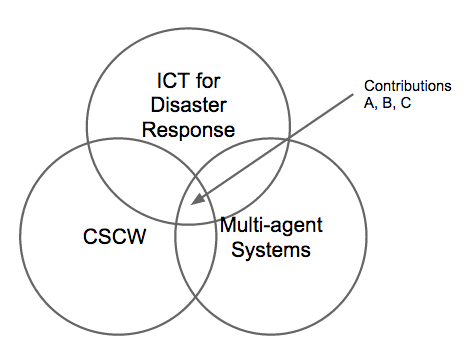
\includegraphics[scale=0.5]{img/introduction/contributions.png}
  \caption{contributions}
  \label{fig:contributions}
\end{figure}


This thesis contributes to the knowledge in the following areas (Figure \ref{fig:contributions}): \\

\begin{enumerate}
  \item[A] \textbf{The system prototypes.} Real-world interactive prototypes (i.e. AtomicOrchid) for investigating human-system interaction in a disaster response settings. An iterative prototyping process is conducted throughout the three AtomicOrchid studies, which results in interactive prototypes of planning support systems. 
  
  \item[B] \textbf{The observations.} The field observation of serious game trials generate thick descriptions of human system interaction in the work settings of \ac{DR}. The key observations lead to both interactional issues and detailed system requirements which inspire system evolution across the three trials.
  
  \item[C] \textbf{The interactional issues and design implications.} For each study, field observations are further analysed to enrich our understanding of interactional issues surrounding automated planning support, and generate design implications which contribute to future deployment of automated planning support system in the complex collaborative work setting of \ac{DR}. 
\end{enumerate}


\section{Publications of this thesis} 
Parts of the contents of this thesis have been accepted by peer-review for publication in journal and conference proceedings in the field of \ac{HCI} and multi-agent system or are in submission. The core contributions include: \\


\begin{enumerate}
\item The chapters \ref{ch:approach}, \ref{ch:methodology}  present the approach and methodology employed to study interactional issues of planning support system. Some of the ideas of these chapters expands on the contents in:\\
\texttt{ \footnotesize Fischer, Joel E., \textbf{Wenchao Jiang}, and Stuart Moran. AtomicOrchid: a mixed reality game to investigate coordination in disaster response." In Entertainment Computing-ICEC 2012, pp. 572-577. Springer Berlin Heidelberg, 2012.}\\

\item The exploration of requirements for building coordination support system in chapter \ref{ch:studyone}  has been published in:\\
\texttt{ \footnotesize Fischer, J.E., \textbf{Jiang, W.}, Kerne, A., Greenhalgh, C., Ramchurn, S.D., Reece, S., Pantidi, N. and Rodden, T. (2014). Supporting Team Coordination on the Ground: Requirements from a Mixed Reality Game. To appear in: Proc. 11th Int. Conference on the Design of Cooperative Systems (COOP 14). Springer.}\\


\item The exploration of interactional issues related to human ``On the loop'' pattern reported in chapter \ref{ch:studytwo} has been published in:\\
\texttt{ \footnotesize\textbf{Jiang, W.}, Fischer, J.E., Greenhalgh, C., Ramchurn, S.D., Wu, F., Jennings, N.R. and Rodden, T. (2014). Social Implications of Agent-based Planning Support for Human Teams.  In: Proc. of the 2014 Int. Conference on Collaboration Technologies and Systems (CTS 14). IEEE.}

\item The exploration of interactional issues related to human ``In the loop'' pattern reported chapter \ref{ch:studythree} have been submitted as:\\



\end{enumerate}

Other contributions include:

\begin{enumerate}
\item Some results from studies in chapter \ref{ch:studyone} and \ref{ch:studytwo} also appeals in the journal article:\\
\texttt{ \footnotesize Ramchurn, S. D., Wu, F., Fischer, J. E., Reece, S., \textbf{Jiang, W.}, and Roberts, S. J., et al. (2015). Human-agent collaboration for disaster response. Journal of Autonomous Agents and Multi-Agent Systems.}\\

\item The game probe `AtomicOrchid' built in this PhD work is a central component of HAC-ER (Human Agent Collectives for Emergency Response) system  developed as main demonstrator of ORCHID project (orchid.ac.uk). The demonstrator is presented in the paper:\\
\texttt{ \footnotesize Ramchurn, S. D., Simpson, E., Fischer, J. E., Huynh, D. T., Ikuno, Y., Reece, S., and \textbf{ Jiang, W.} et al. (2015). HAC-ER: A disaster response system based on human-agent collectives. In AAMAS-15 : 14th Int. Conf. on Autonomous Agents and Multi-Agent Systems.} \\ 

\item The planner agent integrated in `AtomicOrchid' is based on a novel multi-agent coordination algorithm. Evaluation of the algorithm is partially facilitated the 'AtomicOrchid' trials:\\
 \texttt{ \footnotesize Wu, F., Ramchurn, S. D., \textbf{Jiang, W.}, Fischer, J. E., Rodden, T., and Jennings, N. R. (2015). Agile Planning for Real-World Disaster Response. In International Joint Conference on Artifical Intelligence.}

\end{enumerate} 

\section{Structure of the Thesis}
This thesis is structured as four parts. Part I surveys the relevant background literature. Chapter \ref{ch:literatures} will firstly give an overview of task planning activities together with command and control structures of \ac{DR} teams, followed by a review of empirical studies related to command and control work settings. The Chapter \ref{ch:literatures} then examines the state-of-the-art technology practices from 3 perspectives including planning support systems, \ac{ICT} support, and application of Artificial Intelligence in \ac{DR}. In Chapter \ref{ch:humanSysRelationship}, the relationship between technological support and human operators will also be examined by reviewing relevant literatures of \ac{CSCW} systems, Automation design and Human agent interactions. The rest of the chapter give an overview of serious mixed reality games which underpins the research approach of this PhD work.\\

Part II develops the approach and methodology employed to study interactional issues with planning support system in two chapters. Chapter \ref{ch:approach} develops the framework of interaction patterns under which interactional issues can be explored. The rest of this chapter introduces serious mixed reality game as approach to study interactions, followed by detailed description of the game used as testbed for this study, AtomicOrchid. Chapter \ref{ch:methodology} describes the methodology used to study the interactional issues. In particular, this chapter describes ethnographic observation and interaction analysis, which is supplemented by interviews. \\ 

Part III presents observational studies of this thesis. Chapter \ref{ch:studyone} reports the first observational study with AtomicOrchid. This version of AtomicOrchid does not have planning support agent included. The study establishes baseline human performance of task planning and derives general requirements of communication support. The Chapter \ref{ch:studytwo} gives an account of the second observational study of AtomicOrchid. In this study, a planning agent was built into the game with the human-on-the-loop interactional arrangement. Chaper \ref{ch:studythree} reports the third field study of AtomicOrchid with the human-in-the-loop arrangement. \\ 

The Part IV chapter \ref{ch:conclusion} concludes this thesis with a summary of discoveries, contributions, limitations and future work.\\









